\documentclass{beamer}
\usetheme{default}
\usepackage{hyperref}
\usepackage{listings}
\lstset{language=Python,
        stringstyle=\ttfamily}

\usepackage{color}
\title{Software Testing Lecture 2 \\ Introduction to Unit Testing and TDD}
\author{Justin Pearson}
\date{2019}
\setbeamertemplate{footline}[page number]
\setbeamertemplate{navigation symbols}{}
\begin{document}
\begin{frame}
  \maketitle
\end{frame}
\begin{frame}
  \frametitle{Unit Testing}
  \begin{itemize}
  \item xUnit testing is a framework where individual functions and
    methods are tested. 
  \item It is not particularly well suited to integration testing or
    regression testing.
  \item The best way to write testable code is to write the tests as
    you develop the code. 
  \item Writing the test cases after the code takes more time and
    effort than writing the test during the code. It is like good
    documentation; you'll always find something else to do if you leave
    until after you've written the code.  
  \end{itemize}
  This will be covered in more detail in the next lecture.
\end{frame}
\begin{frame}
  \frametitle{The heart of Unit Testing}

  The unit test framework is quite powerful. But the heart are two
  functions:
  \begin{itemize}
  \item {\bf assertTrue} 
  \item {\bf assertFalse}
  \end{itemize}
\end{frame}

\begin{frame}
  \frametitle{{\tt assertTrue}}
 Suppose we want to test our string length function {\tt int
   istrlen(char*) }
Then, the following things should be true:
\begin{itemize}
\item The length of {\tt "Hello"} is 5.
\item The length of {\tt ""} is 0.
\item The length of {\tt "My kingdom for a horse."} is 23.
\end{itemize}
\end{frame}
\begin{frame}
  \frametitle{{\tt assertTrue}}
Then we would assert that the following things are true:
\begin{itemize}
\item {\tt assertTrue} (The length of {\tt "Hello"} is 5.)
\item  {\tt assertTrue}(The length of {\tt ""} is 0.)
\item  {\tt assertTrue} (The length of {\tt "My kingdom for a horse."}
  is 23.)
\end{itemize}
\end{frame}

\begin{frame}
  \frametitle{{\tt assertTrue}}
  \begin{itemize}
  \item Key idea in xUnit:
  \item {\tt assertTrue}( executable code )
    \begin{itemize}
    \item  Runs the executable code which should evaluate to true.
    \end{itemize}
  \item {\tt assertFalse}( executable code)

    \begin{itemize}
  \item Runs the executable code which should evaluate to false. 
\end{itemize}
    \end{itemize}
\end{frame}
\begin{frame}
  \begin{itemize}
  \item Different xUnit frameworks run the tests in different
  ways. 
\item Python unit testing framework has a notion of test suites and
  registries.
\item But it is quite simple to set up tests.
\item  Key to success in understanding complex APIs. Take example code
  and modify it to do what you want. 
  \end{itemize}
\end{frame}

\begin{frame}[fragile]
  \frametitle{Python Unit Testing}
\begin{lstlisting}
import code_to_be_tested
import unittest
class TestCode(unittest.TestCase):
   def tests(self):
     x = "Hello"
     self.assertTrue(len(x) == 5)
\end{lstlisting}
\end{frame} 
\begin{frame}
  \frametitle{Important Unit Testing Concepts}
  \begin{itemize}
  \item Setup. You might need to initialise some data structures.  \pause
  \item The tests. Well, you need to do tests. \pause
  \item Teardown. Always! clean up after you. \pause
  \end{itemize}
Important idea.
\begin{itemize}
\item Each test should be able to be run independently of the other
  tests. You don't know in what order the tests will be run. Or even if
  all tests will be run. The programmer might just rerun the test that
  caused problems. 
\end{itemize}
\end{frame}
\begin{frame}
  \frametitle{Teardown}
  \begin{itemize}
  \item Teardown is more common in languages without automatic garbage
    collection. 
  \end{itemize}
\end{frame}

\begin{frame}
\frametitle{Test Driven Development}
\begin{itemize}
\item Test driven development (TDD) is a way of programming where all
  your development is driven by tests.
\item Write tests before you write code. 
\item Only write code when you fail a test. 
\end{itemize}
  \end{frame}
\begin{frame}
\frametitle{The TDD Mantra}
\begin{itemize}
\item \textcolor{red}{Red}: Write a test that fails.
\item \textcolor{green}{Green}: Write code that passes the test.
\item Refactor: If possible refactor your code.
\end{itemize}
It seems a bit counter intuitive at first. I must think about the
algorithm, not the tests. Can I write complex algorithms this way?  
\end{frame}
\begin{frame}
  \frametitle{TDD}
  \begin{itemize}
  \item The key is to start small. Simple tests.
  \item Grow your code slowly. 
  \item Only make your code more complex if the tests require it.
  \item Think of a good sequence of tests.
  \end{itemize}
\end{frame}
\begin{frame}
  \frametitle{Two Examples}
  \begin{itemize}
  \item Converting numbers to English.
  \item A score board for the game of darts.
%  \item Part of  parser for bibtex entries.
  \end{itemize}
\end{frame}
\begin{frame}
  \frametitle{Refactoring}
  \begin{itemize}
  \item For us, refactoring will be taking a piece of code and making
    it simpler to understand and smaller. Hopefully it makes it more
    efficient. Although we won't worry too much about
    efficiency. Clear, readable code is our goal. Efficiency comes when
    it is needed.
  \item ``We should forget about small efficiencies, say about 97\% of
    the time: premature optimization is the root of all evil.'' Donald Knuth.
  \item When you start doing OO design, then refactoring  also means
    tinkering with the object hierarchy.
  \end{itemize}
\end{frame}
\begin{frame}
  \frametitle{{\tt toEnglish}}

  \begin{itemize}
  \item  The idea is to write a function that given a number between 0 and 999
inclusive returns a string spelling out the number in English. For
example {\tt toEnglish(43)} should produce the string {\tt 'forty
  three'}. 
\item We are going to develop the function in Python. If you are
not familiar with Python, then  pretend it is pseudo code.
\item See the web page for accompanying pdf file that explains how to
  set up the tests. 
  \end{itemize}
\end{frame}
\begin{frame}[fragile]
  \frametitle{Red}
  First let us  write a test that will fail.
  \color{red}
\begin{lstlisting}
  assertEqual(toEnglish.toEnglish(0),'zero')
\end{lstlisting}
\color{black}
Apart from setting up the minimal amount of files to get the modules
going we have no code. This test will fail.
\end{frame}
\begin{frame}[fragile]
  \frametitle{Green}
  \begin{itemize}
  \item Do not think ahead. Write the minimal code that will pass the test.
  \end{itemize}
  \begin{lstlisting}
   def toEnglish(n):
    return('zero')
  \end{lstlisting}
Stupid? Well it gets us going.
\end{frame}
\begin{frame}[fragile]
\frametitle{Red}
We need to find a test that fails.
\color{red}
\begin{lstlisting}
     assertEqual(toEnglish.toEnglish(1),'one')
   \end{lstlisting}
\color{black}
This test of course fails.
\begin{verbatim}
self.assertEqual(toEnglish.toEnglish(1),'one')
AssertionError: 'zero' != 'one'
\end{verbatim}
\end{frame}
\begin{frame}[fragile]
  \frametitle{Green}
Write the minimum to pass the test.
\begin{lstlisting}
  def toEnglish(n):
    if   n==0:
        return('zero')
    elif n==1:
        return('one')
\end{lstlisting}
Now all the tests pass. {\tt elif} is short for {\tt else if}
\end{frame}

\begin{frame}[fragile]
\frametitle{Red}
You can see where this is going.
\color{red}
  \begin{lstlisting}
assertEqual(toEnglish.toEnglish(2),'two')
\end{lstlisting}
\color{black}
\end{frame}

\begin{frame}[fragile]
\frametitle{Green}
\begin{lstlisting}
def toEnglish(n):
    if   n==0:
        return('zero')
    elif n==1:
        return('one')
    elif n==2:
        return('two')
\end{lstlisting}
\end{frame}
\begin{frame}[fragile]
 We are on a  roll. We understand our tests and understand our
 code. This will not go on for ever, but it is a start.
  \begin{lstlisting}
assertEqual(toEnglish.toEnglish(3),'three')
assertEqual(toEnglish.toEnglish(4),'four')
assertEqual(toEnglish.toEnglish(5),'five')
assertEqual(toEnglish.toEnglish(6),'six')
assertEqual(toEnglish.toEnglish(7),'seven')
assertEqual(toEnglish.toEnglish(8),'eight')
assertEqual(toEnglish.toEnglish(9),'nine')
assertEqual(toEnglish.toEnglish(10),'ten')
assertEqual(toEnglish.toEnglish(11),'eleven')
\end{lstlisting}
\end{frame}
\begin{frame}[fragile]
You can guess what the code looks like.
\begin{lstlisting}
    def toEnglish(n):
    if   n==0:
        return('zero')
    elif n==1:
        return('one')
    elif n==2:
        return('two')
    elif n==3:
        return('three')
    elif n==4:
        return('four')
    elif n==5:
     ....... 
\end{lstlisting}
\end{frame}
\begin{frame}[fragile]
\frametitle{Refactor}
Now we are being too slow and stupid. Refactor. Use a list instead of
a bunch of {\tt if} statements.
\begin{lstlisting}
  def toEnglish(n):
    numbers = ['zero','one','two','three','four',
               'five','six','seven','eight',
               'nine','ten','eleven']
    return(numbers[n])
\end{lstlisting}
Rerun the tests to make sure that your refactoring does not mess
anything up.
\end{frame}
\begin{frame}[fragile]
\frametitle{Red}
We need to find tests that fail. While we know what is going on we
take bigger steps. 
\begin{lstlisting}
assertEqual(toEnglish.toEnglish(12),'twelve')	
assertEqual(toEnglish.toEnglish(13),'thirteen')	
assertEqual(toEnglish.toEnglish(14),'fourteen')
assertEqual(toEnglish.toEnglish(15),'fifteen')
assertEqual(toEnglish.toEnglish(16),'sixteen')
assertEqual(toEnglish.toEnglish(17),'seventeen')
assertEqual(toEnglish.toEnglish(18),'eighteen')
assertEqual(toEnglish.toEnglish(19),'nineteen')
assertEqual(toEnglish.toEnglish(20),'twenty')
assertEqual(toEnglish.toEnglish(21),'twenty one')
\end{lstlisting}
\end{frame}
\begin{frame}[fragile]
\frametitle{Green}
Well the code should be no surprise.
\begin{lstlisting}
  def toEnglish(n):
    numbers = ['zero','one','two','three','four',
               'five','six','seven','eight',
               'nine','ten','eleven','twelve',
               'thirteen','fourteen','fifteen',
               'sixteen','seventeen','eighteen',
               'nineteen','twenty','twenty one']
    return(numbers[n])
\end{lstlisting}
\end{frame}
\begin{frame}[fragile]
\frametitle{Refactor}
  Time to refactor {\tt 'twenty one'} 
 is {\tt 'twenty' + ' ' + 'one'}. This gives us the  following code:
\begin{lstlisting}
  def toEnglish(n):
    numbers = ['zero','one','two','three','four',
               'five','six','seven','eight',
               'nine','ten','eleven','twelve',
               'thirteen','fourteen','fifteen',
               'sixteen','seventeen','eighteen',
               'nineteen','twenty']
    if n in range(0,20):
        return(numbers[n])
    else:
        return('twenty' + ' ' + numbers[n-20])
\end{lstlisting}
\end{frame}
\begin{frame}[fragile]
\frametitle{Refactor}
  Don't forget to rerun your tests.
\begin{verbatim}
  File "test_toEnglish.py", line 27, in test_simple
    self.assertEqual(toEnglish.toEnglish(20),'twenty')
AssertionError: 'twenty zero' != 'twenty'
\end{verbatim}
Studying the code gives us an error. I had assumed that {\tt
  range(0,20)} produced all the numbers up to and including twenty. It
only goes up to 19. It is in the manual, but I found out by
testing.
\end{frame}
\begin{frame}[fragile]
\frametitle{Refactor --- New version}
\begin{lstlisting}
  def toEnglish(n):
    numbers = ['zero','one','two','three','four',
               'five','six','seven','eight',
               'nine','ten','eleven','twelve',
               'thirteen','fourteen','fifteen',
               'sixteen','seventeen','eighteen',
               'nineteen','twenty']
    if n in range(0,21):
        return(numbers[n])
    else:
        return('twenty' + ' ' + numbers[n-20])
\end{lstlisting}
  Now all the tests work.
\end{frame}
\begin{frame}[fragile]
\frametitle{Red?}
Well now that we have a feel for our problem we can start generating
the test cases in larger steps.
\begin{lstlisting}
assertEqual(toEnglish.toEnglish(22),'twenty two')
assertEqual(toEnglish.toEnglish(23),'twenty three')
assertEqual(toEnglish.toEnglish(29),'twenty nine')
\end{lstlisting}
Well we still are not at our red state because all our tests are
passed.
\end{frame}
\begin{frame}[fragile]
\frametitle{Red}
\begin{lstlisting}
assertEqual(toEnglish.toEnglish(30),'thirty')
\end{lstlisting}
Now we fail.
\begin{verbatim}
  File "test_toEnglish.py", line 32, in test_simple
    self.assertEqual(toEnglish.toEnglish(30),'thirty')
AssertionError: 'twenty ten' != 'thirty'
\end{verbatim}  
\end{frame}
\begin{frame}[fragile]
  \frametitle{Green}
So thirty should be treated as a special case.
\begin{lstlisting}
  def toEnglish(n):
    numbers = [ .... ]
    if n in range(0,21):
        return(numbers[n])
    elif n in range(21,30):
        return('twenty' + ' ' + numbers[n-20])
    elif n == 30 :
        return('thirty')
    elif n in range(31,40):
        return('thirty' + ' ' + numbers[n-30])
\end{lstlisting}
\end{frame}
\begin{frame}[fragile]
\frametitle{Red}
All is still going well; tests are passing. 
\begin{lstlisting}
assertEqual(toEnglish.toEnglish(32),'thirty two')
assertEqual(toEnglish.toEnglish(39),'thirty nine')
\end{lstlisting}
Our goal is to find tests that fail. Don't develop any code until you
can find a test that fails.
\begin{lstlisting}
assertEqual(toEnglish.toEnglish(40),'forty')
assertEqual(toEnglish.toEnglish(41),'forty one')
assertEqual(toEnglish.toEnglish(49),'forty nine')
\end{lstlisting}
\end{frame}
\begin{frame}[fragile]
  \frametitle{Green}
\begin{lstlisting}
  def toEnglish(n):
    numbers = [ .... ]
    if n in range(0,21):
        return(numbers[n])
    elif n in range(21,30):
        return('twenty' + ' ' + numbers[n-20])
    elif n == 30 :
        return('thirty')
    elif n in range(31,40):
        return('thirty' + ' ' + numbers[n-30])
    elif n == 40:
        return('forty')
    elif n in range(41,50):
        return('forty' + ' ' + numbers[n-40])
\end{lstlisting}
\end{frame}
\begin{frame}[fragile]
\frametitle{Refactor}
Now time to refactor. Looking at the code, we can use a similar trick
with a list instead of all those {\tt if} statements.
\begin{lstlisting}
  def toEnglish(n):
    numbers = [...]
    tens = ['twenty','thirty','forty','fifty',
            'sixty','seventy','eighty','ninety']
    numberOfTens  = n // 10
    numberOfUnits = n % 10
    if n in range(0,20):
        return(numbers[n])
    return_string = tens[numberOfTens]
    if numberOfUnits > 0 :
        return_string += ' ' \
                         + numbers[numberOfUnits]
    return(return_string)
\end{lstlisting}
\end{frame}
\begin{frame}[fragile]
  \frametitle{Refactor}
Running the tests, we have to see if we didn't mess anything up.
\begin{verbatim}
  File "test_toEnglish.py", line 27, in test_simple
    self.assertEqual(toEnglish.toEnglish(20),'twenty')
AssertionError: 'forty' != 'twenty'
\end{verbatim}
Problem with the {\tt tens} list. I got the indexing wrong. One way to
fix it is to add two dummy values at the head of the list.
\end{frame}
\begin{frame}[fragile]
\frametitle{Refactor}
\begin{lstlisting}
  def toEnglish(n):
    numbers = [...]
    tens = ['','','twenty','thirty','forty','fifty',
            'sixty','seventy','eighty','ninety']
    numberOfTens  = n // 10
    numberOfUnits = n % 10
    if n in range(0,20):
        return(numbers[n])
    return_string = tens[numberOfTens]
    if numberOfUnits > 0 :
        return_string += ' ' \
                         + numbers[numberOfUnits]
    return(return_string)
\end{lstlisting}  
Now all the tests pass.
\end{frame}
\begin{frame}[fragile]
\frametitle{Red}
When adding more tests we don't need to add one for every value between
zero and ninety nine, but we need to check border cases. We are still
looking for test that make our code fail so we can write some code.
\begin{lstlisting}
assertEqual(toEnglish.toEnglish(100),'one hundred')
\end{lstlisting}
\end{frame}
\begin{frame}[fragile]
So, we rewrite the code with the minimal effort to pass the test (it
was late in the day).
\begin{lstlisting}
  def toEnglish(n):
    numbers = [...]
    tens = [..] 
    numberOfTens  = n // 10
    numberOfUnits = n % 10
    if n in range(0,20):
        return(numbers[n])
    elif numberOfTens in range(1,10):
        return_string = tens[numberOfTens]
        if numberOfUnits > 0 :
            return_string += 
             ' '+numbers[numberOfUnits]
        return(return_string)
    return('one hundred')
\end{lstlisting}
\end{frame}
\begin{frame}[fragile]
\frametitle{Red}
If we add the test
\begin{lstlisting}
assertEqual(toEnglish.toEnglish(200),'two hundred')
\end{lstlisting}
then the code will fail and we will have to rewrite something.
\end{frame}
\begin{frame}[fragile]
\frametitle{Green}
\begin{lstlisting}[basicstyle=\fontsize{9}{9}\selectfont]
  def toEnglish(n):
    numberOfHundreds = n // 100
    numberOfTens  = n // 10
    numberOfUnits = n % 10
    return_string = ''
    if n in range(0,20):
        return(numbers[n])
    elif numberOfHundreds in range(1,10):
        return_string = return_string +\
                    numbers[numberOfHundreds] + ' hundred'
    elif numberOfTens in range(1,10):
        return_string = return_string + tens[numberOfTens]
        if numberOfUnits > 0 :
            return_string += 
             ' ' + numbers[numberOfUnits]
    return(return_string)
\end{lstlisting}

\end{frame}
\begin{frame}[fragile]
  \frametitle{Green/Refactor}
Part of the problem is our \texttt{numberOfTens} calculation assumes that n is
two digits and we got our logic wrong with the elif stuff. But we can
do some refactoring and use \texttt{toEnglish} ourselves using the fact that:
\begin{lstlisting}
 'k*100 + w' = toEnglish(k) +
    'hundred and ' + toEnglish(w)  
\end{lstlisting}

We are cheating a bit by doing the refactoring in one step, but by
doing all these tests we have a deeper understanding of the problem.

\end{frame}
\begin{frame}[fragile]
  \frametitle{Green/Refactor}
\begin{lstlisting}

    elif numberOfHundreds in range(1,10):
        return_string += 
             numbers[numberOfHundreds] + ' hundred'
        n = n - numberOfHundreds*100
        return_string +=  ' and ' + toEnglish(n)
        return(return_string)
    elif numberOfTens in range(1,10):
        return_string += tens[numberOfTens]
        if numberOfUnits > 0 :
            return_string += 
               ' ' + numbers[numberOfUnits]
            return(return_string)
  \end{lstlisting}
\end{frame}

\begin{frame}[fragile]
\frametitle{Green}
Let's run the tests.
\begin{verbatim}

AssertionError: 'one hundred and zero' != 'one hundred'
AssertionError: None != 'twenty'
AssertionError: None != 'thirty'
\end{verbatim}
We seem to have messed up something with the numbers less than one
hundred, but lets just fix the problems one at a time. We'll fix the
{\tt 'one hundred and zero'} problem.
\end{frame}
%
\begin{frame}[fragile]
\frametitle{Green}

\begin{lstlisting}
      elif numberOfHundreds in range(1,10):
        return_string += 
            numbers[numberOfHundreds] + ' hundred'
        n = n - numberOfHundreds*100
        if n>0:
            return_string += ' and ' + toEnglish(n)
        return(return_string)
    elif numberOfTens in range(1,10):
        return_string += tens[numberOfTens]
        if numberOfUnits > 0 :
            return_string += 
              ' ' + numbers[numberOfUnits]
            return(return_string)
\end{lstlisting}
\end{frame}

\begin{frame}[fragile]
  \frametitle{Green}
But we still get the problems with 
\begin{verbatim}
AssertionError: None != 'twenty'

AssertionError: None != 'thirty'
\end{verbatim}
It means that I've got some of the if-then-else logic wrong; an easy
problem in Python. Good job we have got tests to see if we have messed
things up.

Look at the handout for the code. It does not really  fit on a slide.
\end{frame}
\begin{frame}[fragile]
  \begin{lstlisting}[basicstyle=\fontsize{8}{9}\selectfont]
def toEnglish(n):
    numbers = [... ] 
    tens = [...]
    numberOfHundreds = n // 100
    numberOfTens  = n // 10
    numberOfUnits = n % 10
    return_string = ''
    if n in range(0,20):
        return(numbers[n])
    if numberOfHundreds in range(1,10):
        return_string = return_string + numbers[numberOfHundreds] + ' hundred'
        n = n - numberOfHundreds*100
        if n>0:
            return_string = return_string + ' and ' + toEnglish(n)
        return(return_string)
    if numberOfTens in range(1,10):
        return_string = return_string + tens[numberOfTens]
        if numberOfUnits > 0 :
            return_string = return_string + ' ' +\ 
            			numbers[numberOfUnits]
        return(return_string)
  \end{lstlisting}
\end{frame}
\begin{frame}
\frametitle{Darts}

\begin{center}
    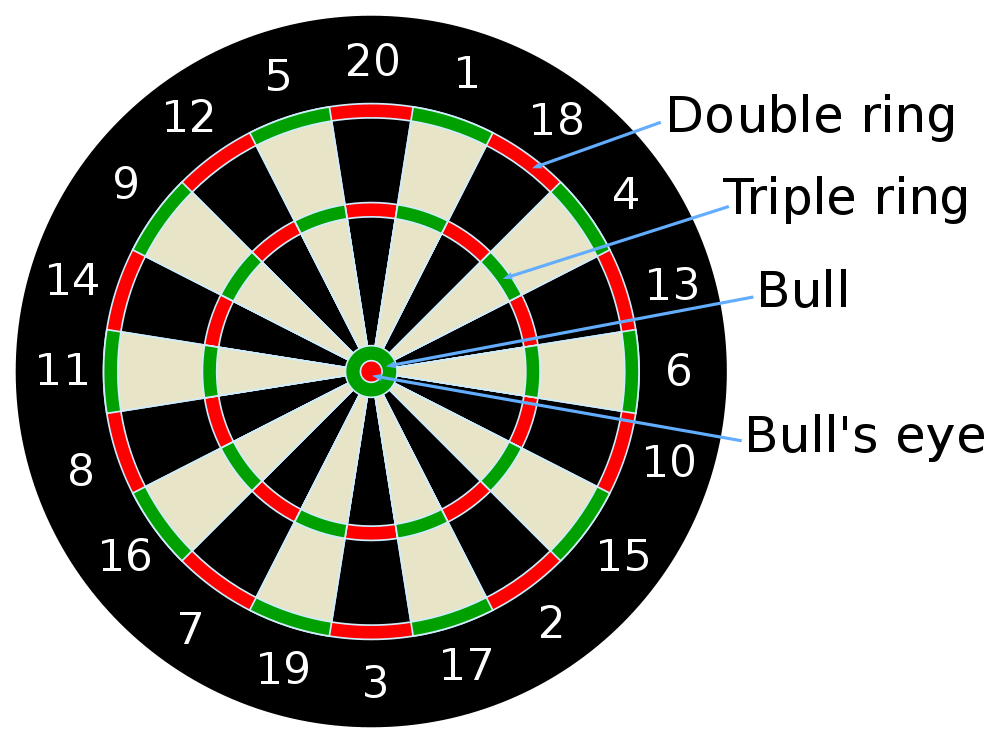
\includegraphics[height=1.86in,width=2.5in]{board.png}
\end{center}
Aim of the game to get your score to exactly 0 counting down from 301. 
\end{frame}
\begin{frame}
  \frametitle{Darts Scoreboard Class}

We will implement a class that keeps track of the score, which
player's turn it is and tells us if somebody has won. In a program
this class would probably be interfaced into a GUI. 
\end{frame}

\begin{frame}[fragile]
  \frametitle{Red}
So the first test we do is to see if we can initialize an object of
the class.

\begin{lstlisting}
   def test_init(self):
        game  = darts.scoreboard()
\end{lstlisting}
This test fails. Since we haven't even written any object code yet.
\end{frame}
\begin{frame}[fragile]
\frametitle{Green}
\begin{lstlisting}
class scoreboard:
    pass
\end{lstlisting}
This class does nothing.  
\end{frame}
\begin{frame}[fragile]
\frametitle{Red}
What do we want to do with the class? It is a two player class. We
want to know the score of player 1 and the score of player 2.

We assume that we are playing pub darts and start at 301. Games take
too long otherwise, and it takes time away from beer.
\begin{lstlisting}
   def test_score(self):
        game  = darts()
        self.assertEqual(game.playerscore(1),301)
        self.assertEqual(game.playerscore(2),301)
\end{lstlisting}
Notice that we are deciding the interfaces to the class by writing the tests.
\end{frame}
\begin{frame}[fragile]
\frametitle{Green}
\begin{lstlisting}
class scoreboard:
    def __init__(self):
        self.playerscores = [301,301]
    def playerscore(self,player):
        return(self.playerscores[player-1])
\end{lstlisting}
The {\tt init} method is called when an object is called.  
\end{frame}
\begin{frame}[fragile]
\frametitle{Red}
We only want two players. We want an exception thrown if we ask for
the score of another player.
\begin{lstlisting}
   def test_exception(self):
        game = darts.scoreboard()
        self.assertRaises(NameError,
                          game.playerscore,3)
\end{lstlisting}
\end{frame}

\begin{frame}[fragile]
\frametitle{Green}
\begin{lstlisting}
      def playerscore(self,player):
        if player == 1 or player == 2:
            return(self.playerscores[player-1])
        else:
            raise NameError('player out of range')
\end{lstlisting}
    
\end{frame}


\begin{frame}[fragile]
A darts board is divided into 20 regions. In each region you can score
a single or double or triple times the score. So we want players to
enter their score.
\begin{lstlisting}
def test_scoring(self):
  game = darts.scoreboard()
  game.playerthrown(1,'single',15)
  self.assertEqual(game.playerscore(1),301-15)
  game.playerthrown(1,'double',20)
  self.assertEqual(game.playerscore(1),301-15-2*20)
  game.playerthrown(1,'triple',5)
  self.assertEqual(game.playerscore(1),
                   301-15-2*20-3*5)
\end{lstlisting}
  
\end{frame}
\begin{frame}[fragile]
The test will fail, as we do not have a {\tt playerthrown} method. So
first attempt is to correct the code.
\begin{lstlisting}
def playerthrown(self,player,multiplier,number):
  if multiplier == 'double':
      number = number*2
  elif multiplier == 'triple':
      number = number*3
  self.playerscores[player-1] += number
\end{lstlisting}
\end{frame}

\begin{frame}[fragile]
At least it runs, but I still fail the test.
\begin{verbatim}
 self.assertEqual(game.playerscore(1),301-15)
   AssertionError: 316 != 286
\end{verbatim}
Did I get the code wrong or the tests wrong. The test looks fine, but
I want to isolate things so I can pinpoint the problem. 
\end{frame}
\begin{frame}[fragile]
\begin{lstlisting}
    def test_scoring_single(self):
        game = darts.scoreboard()
        game.playerthrown(1,'single',15)
        self.assertEqual(game.playerscore(1),
                         301-15)
    def test_scoring_double(self):
        game = darts.scoreboard()
        game.playerthrown(1,'double',20)
        self.assertEqual(game.playerscore(1),
                        301-(2*20))
    def test_scoring_triple(self):
        game = darts.scoreboard()
        game.playerthrown(1,'triple',5)
        self.assertEqual(game.playerscore(1),
                         301-(3*5))
\end{lstlisting}
 All three tests fail.
\end{frame}
\begin{frame}[fragile]
  Looking at the code, I have made a stupid error.
\begin{lstlisting}
       self.playerscores[player-1] += number
\end{lstlisting}
should be
\begin{lstlisting}
       self.playerscores[player-1] -= number
\end{lstlisting}
Now, finally, all the tests pass.
\end{frame}
\begin{frame}[fragile]
\frametitle{Red}
Darts is a two player game. First, player 1 plays three shots then player
two plays three shots. We have to decide how the object behaves if
players play out of turn. We'll throw exceptions. There are other ways
of doing this, but {\em now} is the time to decide. Write the tests to
capture the behaviour that you want. If you want to change the
behaviour later you will have to rewrite the tests.

\end{frame}
\begin{frame}[fragile]
\frametitle{Red}
\begin{lstlisting}
def test_player_1_plays_first(self):
        game = darts.scoreboard()
        #If a player 2 plays before player 1 then raise an exception.
        self.assertRaises(NameError, 
                 game.playerthrown,2,'single',5)   
\end{lstlisting}
Of course the test fails.
  
\end{frame}
\begin{frame}[fragile]
 To solve this problem we need a variable that keeps track of the
 state of who's turn it is. So we modify the {\tt init} method.
 \begin{lstlisting}
 def __init__(self):
     self.playerscores = [301,301]
     self.turn = 1
 \end{lstlisting}
And, modify the {\tt playerthrown} method. 
\begin{lstlisting}
def playerthrown(self,player,multiplier,number):
    if player != turn:
       raise NameError('throw out of turn')
        .....
\end{lstlisting}
\end{frame}
\begin{frame}[fragile]
\frametitle{Green}
Tests still fail. 
\begin{verbatim}
  NameError: global name 'turn' is not defined
\end{verbatim}
I forgot to use {\tt self.turn} instead of {\tt turn}. When it is
fixed all the tests pass.
\end{frame}

\begin{frame}[fragile]
\frametitle{Red}
 Now we have to think about how the game works. 
 You make 3 throws and then it is the other player's turn.

 Since we are using exceptions we expect the following code to be
 exception free.

\begin{lstlisting}
  def test_three_throws(self):
       game = darts.scoreboard()
       game.playerthrown(1,'triple',5)
       game.playerthrown(1,'triple',5)
       game.playerthrown(1,'triple',5)
       game.playerthrown(2,'triple',20)
\end{lstlisting}
When the tests run, we get an exception when player two tries to throw
a dart.  
\end{frame}
\begin{frame}[fragile]
So, we need to keep track of how many throws have been. If we get to 3
then it is the other player's turn.

First modify {\tt init}
\begin{lstlisting}
   def __init__(self):
        self.playerscores = [301,301]
        self.turn = 1
        self.throws = 0
\end{lstlisting}
And, then  modify {\tt playerthrown} to keep track of how many throws and flip the
player when there have been 3 throws.
\begin{lstlisting}
def playerthrown(self,player,multiplier,number):
    if player != self.turn:
         raise NameError('throw out of turn')
    self.throws = self.throws + 1
    if (self.throws == 3):
         self.turn = 1 - self.turn
\end{lstlisting}
  
\end{frame}
\begin{frame}[fragile]
But, the tests still fail.
\begin{verbatim}
======================================================================
ERROR: test_three_throws (__main__.TestDarts)
----------------------------------------------------------------------
Traceback (most recent call last):
  File "/var/folders/rE/rEvVYKXVEFWAJ9IyyNGDqk++42I/-Tmp-/Python3.274950pHt.py", line 38, in test_three_throws
  File "darts.py", line 14, in playerthrown
    raise NameError('throw out of turn')
NameError: throw out of turn

----------------------------------------------------------------------
\end{verbatim}
Ah, I'm stupid. I have a problem with indexing players both by 1 and
by 0. This is going cause more errors in the future. From now on I
will always index the players by 1. So I'll use the trick of having a
dummy entry in the {\tt playerscores} for the index 0 and rewrite the rest
of the code accordingly.
\end{frame}
\begin{frame}[fragile]
\begin{lstlisting}
    def __init__(self):
        self.playerscores = [None,301,301]
        #  turn = 1 or 2 player's turn.    
        self.turn = 1
        self.throws = 0
    def playerscore(self,player):
        if player == 1 or player == 2:
            return(self.playerscores[player])
        else:
            raise NameError('player out of range')
\end{lstlisting}
\end{frame}
\begin{frame}[fragile]
  

\begin{lstlisting}
    def playerthrown(self,player,multiplier,number):
        if player != self.turn:
            raise NameError('throw out of turn')
        self.throws = self.throws + 1
        if (self.throws == 3):
            if (self.turn == 1):
                self.turn = 2
            else:
                self.turn = 1
        if multiplier == 'double':
              number = number*2
        elif multiplier == 'triple':
            number = number*3
        self.playerscores[player] -= number
\end{lstlisting}
  
\end{frame}

\begin{frame}[fragile]
\frametitle{Red}
Lets extend the previous test to make sure that we have got the logic
of turns and throws correct.
\begin{lstlisting}
def test_three_throws(self):
  game = darts.scoreboard()
  game.playerthrown(1,'triple',5)
  game.playerthrown(1,'triple',5)
  game.playerthrown(1,'triple',5)
  game.playerthrown(2,'triple',20)
  game.playerthrown(2,'triple',20)
  game.playerthrown(2,'triple',20)
  game.playerthrown(1,'triple',20)
  self.assertEqual(game.playerscore(1),301-3*(3*5) - 3*20)
  self.assertEqual(game.playerscore(2),301-3*20)
\end{lstlisting}

  
\end{frame}
\begin{frame}[fragile]
The tests still fail.

\begin{verbatim}
====================================================
ERROR: test_three_throws (__main__.TestDarts)
----------------------------------------------------
Traceback (most recent call last):

  File "darts.py", line 16, in playerthrown
    raise NameError('throw out of turn')
NameError: throw out of turn
\end{verbatim}

Looking at the
code, I've forgotten to reset the number of throws.
  
\end{frame}
\begin{frame}[fragile]
\frametitle{Green}
\begin{lstlisting}
def playerthrown(self,player,multiplier,number):
   if player != self.turn:
       raise NameError('throw out of turn')
   self.throws = self.throws + 1
   if (self.throws == 3):
      self.throws = 0
      if (self.turn == 1):
          self.turn = 2
      else:
          self.turn = 1
   if multiplier == 'double':
       number = number*2
   elif multiplier == 'triple':
      number = number*3
   self.playerscores[player] -= number
\end{lstlisting}
\end{frame}
\begin{frame}[fragile]
Well the last test still fails.
\begin{verbatim}
  File "/var/folders/rE/rEvVYKXVEFWAJ9IyyNGDqk++42I/-Tmp-/Python3.274950C3C.py", line 57, in test_three_throws_3
AssertionError: 121 != 241
\end{verbatim}
Is it the code or the test? I've miscalculated the score.
This test is getting a bit complicated. We've tested the scoring
system for  player 1. So lets divide the test up a bit.
\end{frame}
\begin{frame}[fragile]
\begin{lstlisting}
def test_three_throws_3(self):
   game = darts.scoreboard()
   game.playerthrown(1,'double',5)
   game.playerthrown(1,'double',5)
   game.playerthrown(1,'double',5)
   game.playerthrown(2,'triple',20)
   game.playerthrown(2,'triple',20)
   game.playerthrown(2,'triple',20)
   self.assertEqual(game.playerscore(2),301-3*20)
\end{lstlisting}
The test still fails.
\begin{verbatim}
AssertionError: 121 != 241
\end{verbatim}
\end{frame}
\begin{frame}[fragile]
Why do we get the answer 121? Because it is the right answer. I got
the test wrong.
\begin{lstlisting}
def test_three_throws_3(self):
   game = darts.scoreboard()
   game.playerthrown(1,'double',5)
   game.playerthrown(1,'double',5)
   game.playerthrown(1,'double',5)
   game.playerthrown(2,'triple',20)
   game.playerthrown(2,'triple',20)
   game.playerthrown(2,'triple',20)
   self.assertEqual(game.playerscore(2),301-3*3*20)
\end{lstlisting}
Now the tests pass.  
\end{frame}
\begin{frame}
\frametitle{Hunting for Red}
If you look in the handout, there are more examples of tests of the
scoring system.

Now I'm confident that the scoring code works and the players turn
works. You have to stare at the code and think. \newline TDD means you only
have to think about little things at a time. \newline Remember that passing a
bunch of tests does not mean that your code is bug free, you have to
think if you can move on.
  
\end{frame}
\begin{frame}
\frametitle{The end of a darts game}
What happens when you finish a game of darts? The are variations in
rule sets, but the version I played in the pub is that you must finish
on exactly 0.  Also, you must score every throw. I'm not sure what the
real rules are. Anyway, this is a quick way for player 1 to get to 0.
\end{frame}
\begin{frame}[fragile]
\begin{lstlisting}
def test_win(self):
   game = darts.scoreboard()
   game.playerthrown(1,'triple',20)
   game.playerthrown(1,'triple',20)
   game.playerthrown(1,'triple',20)
   game.playerthrown(2,'single',1)
   game.playerthrown(2,'single',1)
   game.playerthrown(2,'single',1)
   game.playerthrown(1,'double',19)
   game.playerthrown(1,'double',19)
   game.playerthrown(1,'double',19)
   game.playerthrown(2,'single',1)
   game.playerthrown(2,'single',1)
   game.playerthrown(2,'single',1)
   game.playerthrown(1,'single',1)
   game.playerthrown(1,'single',3)
   game.playerthrown(1,'single',3)
   self.assertEqual(game.playerscore(1),0)  
\end{lstlisting}
\end{frame}

\begin{frame}
\frametitle{Red?}
\begin{itemize}
\item Well we still have not reached condition red. This test passes. We
have to decide what we want the class to do when a player wins. 
The alternatives are  Exceptions, or  Special value for the score?
\item Personally I like using exceptions for non-error conditions, but some
people think this is a bad idea. On some languages exceptions also
carry unnecessary extra overhead. So, since this scoreboard will
probably be interfaced to a GUI, we'll return a string 'WON' when the
score goes to 0.
\end{itemize}
\end{frame}
\begin{frame}[fragile]
So lets modify the last line of the test.
\begin{lstlisting}
self.assertEqual(game.playerscore(1),'WON')  
\end{lstlisting}

The test fails. 
\end{frame}
\begin{frame}[fragile]
\frametitle{Green}
So lets make the score function return 'WON' if the score is 0.
\begin{lstlisting}
def playerscore(self,player):
    if player == 1 or player == 2:
        if (self.playerscores[player] != 0 ): 
            return(self.playerscores[player])
        else:
            return('WON')
    else:
        raise NameError('player out of range')
 \end{lstlisting}
All tests pass.
  
\end{frame}
\begin{frame}[fragile]
\frametitle{Red}
If you get a negative score during a throw then your score is reset
back to what it was before the throw (in some variants you have to end
on a double as well, we won't bother with that).  So we can modify the
previous test.

You can modify the test to make sure that your score is reset each
round. See the handout.

When you run the test you get:
\begin{verbatim}
AssertionError: -64 != 'WON'
\end{verbatim}
  
\end{frame}
\begin{frame}[fragile]
\frametitle{Green}
So we'll need to keep track of the score in the current round.
Modify {\tt init}.
\begin{lstlisting}
   def __init__(self):
        self.playerscores = [None,301,301]
        self.turn = 1
        self.throws = 0
        self.current_round = 0
\end{lstlisting}
When we flip the current player we'll check if the score is negative. If it
is, then we'll add the {\tt current\_round} score back to the score so the
score should be reset to the score before the round.
  
\end{frame}

\begin{frame}[fragile]
\frametitle{Green}
\begin{lstlisting}
  def playerthrown(self,player,multiplier,number):
        if player != self.turn:
            raise NameError('throw out of turn')
        self.throws = self.throws + 1
        if (self.throws == 3):
            self.throws = 0
            if self.playerscores[player] < 0:
                self.playerscores[player] += 
                  self.current_round                
            self.current_round = 0
            if (self.turn == 1):
                self.turn = 2
            else:
                self.turn = 1
         ...... 
        self.playerscores[player] -= number
        self.current_round += number
\end{lstlisting}
  
\end{frame}
\begin{frame}[fragile]
The test still fails.
\begin{verbatim}
FAIL: test_win_2 (__main__.TestDarts)
----------------------------------------------------------------------
Traceback (most recent call last):
  File "/var/folders/rE/rEvVYKXVEFWAJ9IyyNGDqk++42I/-Tmp-/Python3.274950D4J.py", line 126, in test_win_2
AssertionError: -59 != 'WON'

----------------------------------------------------------------------
\end{verbatim}
  
 I must have got the logic wrong for incrementing and decrementing the
score. I got the current round logic wrong. Previously, when I flipped it didn't
affect the rest of the code. Now I have to flip in the right place.
I cheated by adding print statements to see what was going wrong. Old
habits die hard!
\end{frame}
\begin{frame}[fragile]
\begin{lstlisting}
def playerthrown(self,player,multiplier,number):
  if player != self.turn:
      raise NameError('throw out of turn')
  self.throws = self.throws + 1
    ......  Numbers stuff
  self.playerscores[player] -= number
  self.current_round += number
  if (self.throws == 3):
      self.throws = 0
      if (self.turn == 1):
          self.turn = 2
      else:
          self.turn = 1
      if self.playerscores[player] < 0:
           self.playerscores[player] +=
                self.current_round
       self.current_round = 0
\end{lstlisting}
\end{frame}
%
 \begin{frame}
    \frametitle{Working Dart Class}
    \begin{itemize}
    \item Now you have a working dart board class. 
    \item You could extend it with more tests. If you hit the bull you
      get 50 and if you hit the outer bull you get 25. 
    \item Handle non-scoring throws. 
    \item Handle different variants of darts. This might mean that you
      start introducing sub-classing.
    \end{itemize}
 If you are designing a GUI it is good idea to separate logic from the
 GUI stuff. There are various design patterns out there MVC is one
 (Model, View, Controller).
 
  \end{frame}

\end{document}

%%% Local Variables:
%%% mode: latex
%%% TeX-master: t
%%% End:
